%%%%%%%%%%%%%%%%%%%%%%
%%Options for presentations (in-class) and handouts (e.g. print). 
%\documentclass[pdf]{beamer} 
\documentclass[pdf,handout]{beamer}
\usepackage{pgfpages}
\pgfpagesuselayout{2 on 1}[letterpaper,border shrink=5mm]

%%%%%%%%%%%%%%%%%%%%%%
%Change this for different slides so it appears in bar
\usepackage{authoraftertitle}
\date{$\mathbb{R}^n$: Parametric Lines}

%%%%%%%%%%%%%%%%%%%%%%
%% Upload common style file
\usepackage{LyryxLinearAlgebraSlidesStyle}

\begin{document}

%%%%%%%%%%%%%%%%%%%%%%%
%% Title Page and Copyright Common to All Slides

%Title Page
\input frontmatter/titlepage.tex

%LOTS Page
%\input frontmatter/lyryxopentexts.tex

%Copyright Page
\input frontmatter/copyright.tex

%%%%%%%%%%%%%%%%%%%%%%%%%

{\small
\section{Lines in R3}

%-------------- start slide -------------------------------%
\frame{\frametitle{Lines in $R^3$}
\begin{block}{}
Let $P_0$ and $P$ be two (different)
points in $\RR^3$.  
Then there is a unique line $L$ in $\RR^3$ containing these two
points, 
\uncover<2->{
and the vector $\overrightarrow{P_0P}$ is a
\alert{direction vector} for $L$ (since $L$ is parallel to 
$\overrightarrow{P_0P}$).}

\begin{picture}(3.5,0.9)
\uncover<1->{
\put(0.4,0.465){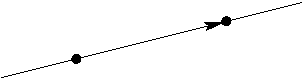
\includegraphics[scale=.7]{figures/vectors-12a.pdf}}
\put(0.3,0.4){\footnotesize $L$}
\put(0.65,0.65){\footnotesize $P_0$}
\put(1.4,0.80){\footnotesize $P$}}
\uncover<2->{
\put(1.0,0.45){\scriptsize \alert{$\overrightarrow{P_0P}$}}
}
\uncover<4->{
\put(2.7,0.1){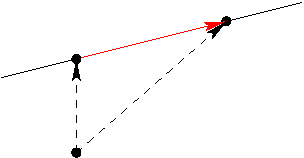
\includegraphics[scale=.7]{figures/vectors-12b.pdf}}
\put(2.6,0.4){\footnotesize $L$}
\put(2.92,0.1){\footnotesize $0$}
\put(2.95,0.65){\footnotesize $P_0$}
\put(3.7,0.80){\footnotesize $P$}
\put(3.25,0.70){\scriptsize $\overrightarrow{P_0P}$}
}
\end{picture}

\uncover<3->{
To describe the line $L$ by an equation, we need to 
specify every point on $L$, and we do this by specifying
the position vector of every point on $L$.}
\uncover<5->{For instance, 
\vspace*{-.1in}

\[ \overrightarrow{0P}=\overrightarrow{0P_0}+\overrightarrow{P_0P}.\]}
\vspace*{-.2in}

\uncover<6->{In fact, if $Q$ is \alert{any point on $L$}, then 
the vector $\overrightarrow{P_0Q}$ is parallel to $\overrightarrow{P_0P}$,
i.e., $\overrightarrow{P_0Q}=t\overrightarrow{P_0P}$ for some $t\in\RR$.}
\uncover<7->{Therefore,
\vspace*{-.1in}

\[ \overrightarrow{0Q}=\overrightarrow{0P_0} +t\overrightarrow{P_0P}.\]}
\vspace*{-.2in}

\uncover<8->{Notice that the point $P$ is used only to get
a vector parallel to the line $L$, i.e., a direction vector for
$L$.}
\end{block}
}
%---------------------- end slide -------------------------%



%---------------------- start slide -----------------------%
\frame{
\begin{block}{The Vector Equation of a Line}
For a line $L$ in $\RR^3$ containing a point
$P_0=(x_0, y_0, z_0)$ and having direction vector
$\vec{d} =\left[\begin{array}{c}
a \\ b \\ c \end{array}\right]$,
\pause

\begin{picture}(3.5,0.7)
\put(1.7,0.1){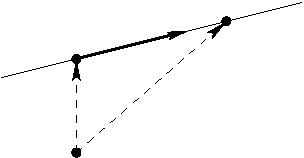
\includegraphics[scale=.7]{figures/vectors-12.pdf}}
\put(1.6,0.4){\small $L$}
\put(1.8,0.1){\small $0$}
\put(1.8,0.62){\small $P_0$}
\put(2.8,0.60){\small $P$}
\put(2.3,0.7){\small $\vec{d}$}
%\put(0,0.3){\small Then
%$\overrightarrow{0P} =
%\overrightarrow{0P_0} +\overrightarrow{P_0P}$, and
%$\overrightarrow{P_0P}$ is parallel}
%\put(0,0.1){to $\vec{d}$, so $\overrightarrow{P_0P}
%=t\vec{d}$ for some $t\in\RR$.}
\end{picture}

the position vector of an arbitrary point $P=(x,y,z)$ on $L$ is
\[ \overrightarrow{0P} = \overrightarrow{0P_0} +
t\vec{d}, t\in\RR.\]
\pause

With the vectors written in component form, the equation is
\[ \left[\begin{array}{c}
x \\ y \\ z \end{array}\right]
=
\left[\begin{array}{c}
x_0 \\ y_0 \\ z_0 \end{array}\right]
+ t \left[\begin{array}{c}
a \\ b \\ c \end{array}\right], t\in\RR.\]

\end{block}
}
%---------------------- end slide -------------------------%

%---------------------- start slide -----------------------%
\frame{
\begin{definition}
Let $\vec{p_0}$ be the position vector of a point
$(x_0,y_0,z_0)$ in $\RR^3$, let $\vec{d}$ be a 
nonzero vector in $\RR^3$,
\pause
and let \alert{$L$} denote the line containing 
\alert{$(x_0,y_0,z_0)$}
and having  direction vector \alert{$\vec{d}$.}  
\pause
If we denote by $\vec{p}$ the position vector of an
arbitrary point on the line $L$,
\pause
then 
\[ \vec{p}=\vec{p_0}+t\vec{d},~ t\in\RR, \]
is a \alert{vector equation} of the line $L$.
\pause
Writing
$\vec{p}= \left[\begin{array}{c}
x \\ y \\ z \end{array}\right]$ 
and
$\vec{d}= \left[\begin{array}{c}
a \\ b \\ c \end{array}\right]$, 
\pause
\[ \left[\begin{array}{c} x \\ y \\ z \end{array}\right]
=
\left[\begin{array}{c} x_0 \\ y_0 \\ z_0 \end{array}\right]
+t\left[\begin{array}{c} a \\ b \\ c \end{array}\right],~t\in\RR\]
is a vector equation of $L$ written in component form.
\end{definition}
}
%---------------------- end slide -------------------------%

%---------------------- start slide -----------------------%
\frame{\frametitle{Brief Aside: Lines in $\RR^2$}
\begin{block}{}
Given a point $(x_0, y_0)$ is $\RR^2$ and a nonzero vector
$\vec{d}$ in $\RR^2$, 
\pause
the line $L$ containing  $(x_0, y_0)$
and having direction vector $\vec{d}$
has vector equation
\[ \left[\begin{array}{c} x \\ y \end{array}\right]
=
\left[\begin{array}{c} x_0 \\ y_0 \end{array}\right]
+t\left[\begin{array}{c} a \\ b \end{array}\right],~t\in\RR,\]
\pause
\vspace*{-.1in}

where 
$\left[\begin{array}{c}
x \\ y \end{array}\right]$ is the position vector of an
arbitrary point on $L$, and 
$\vec{d}= \left[\begin{array}{c} a \\ b \end{array}\right]$.
\pause

For a fixed (but arbitrary) value of $t$, we get
\vspace*{-.1in}

\[ x=x_0+ta ~\mbox{ and } y=y_0+tb.\]
\vspace*{-.1in}

Since $\vec{d}$ is nonzero, not both $a$ and $b$ are zero.  
\pause
Assume $a\neq 0$.  Then $t=\frac{x-x_0}{a}$.
\pause
Substituting this into $y=y_0+tb$ yields
\pause
\[ y=y_0+\frac{x-x_0}{a} b
\pause 
~~~~~\mbox{ or }~~~~~ y-y_0 = \frac{b}{a}(x-x_0).\]
\pause
You (hopefully) recognize this as the equation of a line
given a point $(x_0,y_0)$ and a slope $\frac{b}{a}$.
\end{block}
}
%---------------------- end slide -------------------------%

%---------------------- start slide -----------------------%
\frame{
\begin{example}
The line in $\RR^3$ containing the point $(-5, 1, 3)$ and 
having direction vector 
\bigskip

$\vec{d}=\left[\begin{array}{r} 2 \\ -1 \\ 7 \end{array}\right]$
\pause
has equation
$\left[\begin{array}{c} x \\ y \\ z \end{array}\right] 
=
\left[\begin{array}{r} -5 \\ 1 \\ 3 \end{array}\right] 
+t \left[\begin{array}{r} 2 \\ -1 \\ 7 \end{array}\right],
~t\in\RR$.
\end{example}
\pause
\begin{alertblock}{An equation of a line is not unique}
In the above example, $\vec{d}$ is a direction vector for $L$.
\pause
However, \alert{any nonzero scalar multiple} of $\vec{d}$ is also
a direction vector for $L$.
\pause
Furthermore,
instead of using the point $(-5,1,3)$, we could use any other point
on $L$.  
\pause
Since $(-3,0,10)$ is a point on $L$ (setting $t=1$ is the above
equation), $L$ is also described by the equation
\[ \left[\begin{array}{c} x \\ y \\ z \end{array}\right] 
=
\left[\begin{array}{r} -3 \\ 0 \\ 10 \end{array}\right] 
+t \left[\begin{array}{r} -4 \\ 2 \\ -14 \end{array}\right],
~t\in\RR. \]
\end{alertblock}
}
%---------------------- end slide -------------------------%

%---------------------- start slide -----------------------%
%---------------------- end slide -------------------------%

%---------------------- start slide -----------------------%
%---------------------- end slide -------------------------%

\section{An equation of a line given two points}
%-------------- start slide -------------------------------%
\frame{\frametitle{An equation of a line given two points}
\begin{example}
Let $L$ be a line in $\RR^3$ containing the points
$P(2,-1,7)$ and $P_0(-3,4,5)$.
\pause
Then a direction vector for $L$ is 
\[\overrightarrow{PP_0} =
\left[\begin{array}{c}
-3 - 2 \\ 4 - (-1) \\ 5 - 7
\end{array}\right]=
\left[\begin{array}{r}
-5 \\ 5 \\ -2
\end{array}\right].\]
\pause
Therefore, a vector equation of $L$ is
\[ \left[\begin{array}{r}
x \\ y \\ z \end{array}\right]
=
\left[\begin{array}{r}
2 \\ -1 \\ 7 \end{array}\right]
+
t \left[\begin{array}{r}
-5 \\ 5 \\ -2 \end{array}\right]. \]
\end{example}
}
%-------------- end slide -------------------------------%

\section{An equation of a line given a point and a parallel line}
%-------------- start slide -------------------------------%
\frame{\frametitle{An equation of a line given a point and a
parallel line}
\begin{problem}\em
Find an equation for the line $L$ through $P(4,-7,1)$ and parallel
to the line $M$ with equation
\[ \left[\begin{array}{r}
x \\ y \\ z \end{array}\right]
=
\left[\begin{array}{r}
1 \\ -1 \\ 1 \end{array}\right]
+
t \left[\begin{array}{r}
2 \\ -5 \\ 3 \end{array}\right]. \]
\end{problem}
\pause
\begin{solution}\em
Any direction vector for $M$ is a direction vector for $L$,
\pause
so
$\left[\begin{array}{r}
2 \\ -5 \\ 3
\end{array}\right]$ is a direction vector for $L$.
\pause
Therefore 
\[
\left[\begin{array}{r}
x \\ y \\ z \end{array}\right]
=
\left[\begin{array}{r}
4 \\ -7 \\ 1 \end{array}\right]
+
t \left[\begin{array}{r}
2 \\ -5 \\ 3 \end{array}\right] \]
is an equation for $L$.
\end{solution}
}
%-------------- end slide -------------------------------%


\section{Parametric equations of a line}
%-------------- start slide -------------------------------%
\frame{\frametitle{Parametric equations of a line}
\begin{definition}
Let $L$ be a line with direction vector
$\vect{d}=\left[ \begin{array}{ccc}
a \\ b \\ c \end{array}\right]$
and containing the point $P_0 = (x_0, y_0, z_0)$. 
\pause
From a vector equation of $L$,
\[ \left[\begin{array}{c} x \\ y \\ z \end{array}\right]
=
\left[\begin{array}{c} x_0 \\ y_0 \\ z_0 \end{array}\right]
+t\left[\begin{array}{c} a \\ b \\ c \end{array}\right]\]
\pause
we obtain
\alert{parametric equations of $L$} given by 
\[ \begin{array}{rcl}
x & = & x_0 + ta \\
y & = & y_0 + tb \\
z & = & z_0 + tc
\end{array},~~ t\in\RR. \]
\end{definition}
}
%-------------- end slide -------------------------------%

\section{The intersection of two lines}
%-------------- start slide -------------------------------%
\frame{\frametitle{The intersection of two lines}
\begin{problem}\em
Given two lines $L_1$ and $L_2$, find the point of intersection,
if it exists.
\vspace*{-.1in}

\[ L_1:
\begin{array}{rcl}
x & = & 3+t \\
y & = & 1-2t \\
z & = & 3+3t
\end{array}
\hspace*{1in}
L_2:
\begin{array}{rcl}
x & = & 4+2s \\
y & = & 6+3s \\
z & = & 1+s
\end{array}\]
\end{problem}
\pause
\begin{solution}\em
\alert{This problem is impossible to solve if you use the
same parameter name in both equations.}
\pause
Lines $L_1$ and $L_2$ intersect if and only if there are values
$s,t\in\RR$ such that
\vspace*{-.3in}

\[ \begin{array}{rcl}
3+t & = & 4 + 2s \\
1-2t & = & 6 + 3s \\
3 + 3t & = & 1 + s
\end{array}\]
\vspace*{-.2in}
\pause
i.e., if and only if the system
\[ \begin{array}{rcl}
2s-t & = & -1 \\
3s + 2t & = & -5 \\
s - 3t & = & 2
\end{array}\]
is consistent.
\end{solution}
}
%-------------- end slide -------------------------------%

%-------------- start slide -------------------------------%
\frame{
\begin{solution}[continued]\em
\[
\left[\begin{array}{rr|r}
2 & -1 & -1 \\
3 & 2 & -5 \\
1 & -3 & 2
\end{array}\right]
\rightarrow \cdots \rightarrow
\left[\begin{array}{rr|r}
1 & 0 & -1 \\
0 & 1 & -1 \\
0 & 0 & 0
\end{array}\right]\]
\pause
Since the system in consistent,
$L_1$ and $L_2$ intersect when $s=-1$ and $t=-1$.
\bigskip

\pause
Using the equation for $L_1$
\[ \begin{array}{rcl}
x & = & 3+t \\
y & = & 1-2t \\
z & = & 3+3t \end{array} \]
\pause
and setting $t=-1$, the point of intersection is
\[ P(3+(-1), 1-2(-1), 3+3(-1)) = P(2,3,0).\]

\pause
{\bf Note.} You can check your work by setting $s=-1$ 
in the equation for $L_2$.
\end{solution}
}
%-------------- end slide -------------------------------%

%-------------- start slide -------------------------------%
\frame{
\begin{problem}\em
Find equation\alert{s} for the \alert{lines} through $P(1,0,1)$ that
meet the line
\[ L:
\left[\begin{array}{r}
x \\ y \\ z \end{array}\right]
=
\left[\begin{array}{r}
1 \\ 2 \\ 0 \end{array}\right]
+
t \left[\begin{array}{r}
2 \\ -1 \\ 2 \end{array}\right] \]
at points distance three from $P_0(1,2,0)$.
\end{problem}
\pause
\begin{solution}\em

\begin{picture}(3.5,1.0)
\put(1.4,0.1){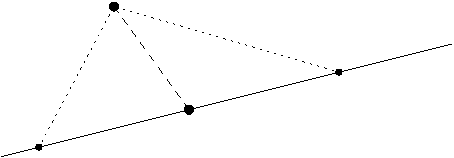
\includegraphics[scale=.7]{figures/vectors-13.pdf}}
\put(1.4,0.2){\small $Q_1$}
\put(2.3,0.2){\small $P_0$}
\put(2.92,0.35){\small $Q_2$}
\put(1.8,0.8){\small $P$}
\end{picture}

Find points $Q_1$ and $Q_2$ on $L$ that are distance three 
from $P_0$, and then find equations for the lines through
$P$ and $Q_1$, and through $P$ and $Q_2$.
\end{solution}
}
%-------------- end slide -------------------------------%

%-------------- start slide -------------------------------%
\frame{
\begin{solution}[continued]\em
\begin{picture}(3.5,1.1)
\put(0.4,0.1){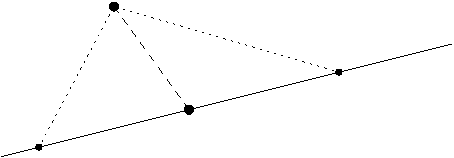
\includegraphics[scale=.7]{figures/vectors-13.pdf}}
\put(0.4,0.2){\small $Q_1$}
\put(1.1,0.1){\small $P_0=(1,2,0)$}
\put(1.92,0.35){\small $Q_2$}
\put(0.7,0.9){\small $P=(1,0,1)$}
\pause
\put(2.7,.4){
$\vec{d}=\left[\begin{array}{r} 2 \\ -1 \\ 2\end{array}\right]$ is a
direction for $L$.}
\end{picture}
\bigskip

\pause
First, $||\vec{d}||=\sqrt{2^2 + (-1)^2 +2^2}=\sqrt{9}=3$,
\pause
so 

\[ \overrightarrow{0Q}_1=\overrightarrow{0P_0} +1\vec{d},
\mbox{ and }~
\overrightarrow{0Q}_2=\overrightarrow{0P_0} -1\vec{d}.\]
\vspace*{-.1in}
\pause
Thus
\[ \overrightarrow{0Q}_1 = 
\left[\begin{array}{r} 1 \\ 2 \\ 0\end{array}\right] +
\left[\begin{array}{r} 2 \\ -1 \\ 2\end{array}\right]
=
\left[\begin{array}{r} 3 \\ 1 \\ 2\end{array}\right]
\pause
\mbox{ and }~
\overrightarrow{0Q}_2 = 
\left[\begin{array}{r} 1 \\ 2 \\ 0\end{array}\right] -
\left[\begin{array}{r} 2 \\ -1 \\ 2\end{array}\right]
=
\left[\begin{array}{r} -1 \\ 3 \\ -2\end{array}\right],
\]
and $Q_1 = (3,1,2)$ and $Q_2=(-1,3,-2)$.
\end{solution}
}
%-------------- end slide -------------------------------%

%-------------- start slide -------------------------------%
\frame{
\begin{solution}[continued]\em
Equations for the lines: 
\begin{itemize}
\item
The line through $P(1,0,1)$ and $Q_1(3,1,2)$ has equation
\pause
\[
\left[\begin{array}{c}
x \\ y \\ z \end{array}\right]
= \overrightarrow{0P}+ t \overrightarrow{PQ}_1
=
\left[\begin{array}{r}
1 \\ 0 \\ 1 \end{array}\right]
+t \left[\begin{array}{r}
2 \\ 1 \\ 1 \end{array}\right]. \]
\pause
\item
The line through $P(1,0,1)$ and $Q_2(-1,3,-2)$ has equation
\[ \left[\begin{array}{c}
x \\ y \\ z \end{array}\right]
= \overrightarrow{0P}+ t \overrightarrow{PQ}_2
= \left[\begin{array}{r}
1 \\ 0 \\ 1 \end{array}\right]
+t \left[\begin{array}{r}
-2 \\ 3 \\ -3 \end{array}\right].  \]
\end{itemize}
\end{solution}
}
%-------------- end slide -------------------------------%

\section{Changing Forms of a Line}
%------------------start slide---------------------------%
\frame{\frametitle{Changing Between Forms of a Line}

\begin{example}
Suppose the \textbf{symmetric form of a line} is
\[
\frac{x-2}{3} = \frac{y-1}{2} = z+3
\]
Find the parametric and vector forms of the line.
\end{example}
\pause
\begin{solution}\em
Let $t = \frac{x-2}{3}$, $t = \frac{y-1}{2}$, and $t= z+3$.
Then, solving for $x, y$ and $z$, we find the parametric equation of the line.
\[
\begin{array}{c}
x = 2+3t \\
y = 1 +2t\\
z = -3 + t
\end{array}
\]
\end{solution}
}
%----------------------end slide--------------------%

%----------------------start slide---------------%
\frame{
\begin{solution}[continued]\em

We can write this in the vector form of the line.
\[
\left[\begin{array}{r}
x \\
y \\
z 
\end{array}
\right]
=
\left[
\begin{array}{r}
2 \\
1 \\
 -3
\end{array} \right]
+ t 
\left[
\begin{array}{r}
3 \\
2 \\
1 
\end{array}\right]
\]
\end{solution}
}
%---------------------end slide----------------------------%

}\end{document}
